
%-----------------------------------------------------------------------------------------------------------------------------------------------%
%	The MIT License (MIT)
%
%	Copyright (c) 2019 Jan Küster
%
%	Permission is hereby granted, free of charge, to any person obtaining a copy
%	of this software and associated documentation files (the "Software"), to deal
%	in the Software without restriction, including without limitation the rights
%	to use, copy, modify, merge, publish, distribute, sublicense, and/or sell
%	copies of the Software, and to permit persons to whom the Software is
%	furnished to do so, subject to the following conditions:
%	
%	THE SOFTWARE IS PROVIDED "AS IS", WITHOUT WARRANTY OF ANY KIND, EXPRESS OR
%	IMPLIED, INCLUDING BUT NOT LIMITED TO THE WARRANTIES OF MERCHANTABILITY,
%	FITNESS FOR A PARTICULAR PURPOSE AND NONINFRINGEMENT. IN NO EVENT SHALL THE
%	AUTHORS OR COPYRIGHT HOLDERS BE LIABLE FOR ANY CLAIM, DAMAGES OR OTHER
%	LIABILITY, WHETHER IN AN ACTION OF CONTRACT, TORT OR OTHERWISE, ARISING FROM,
%	OUT OF OR IN CONNECTION WITH THE SOFTWARE OR THE USE OR OTHER DEALINGS IN
%	THE SOFTWARE.
%	
%
%-----------------------------------------------------------------------------------------------------------------------------------------------%


%============================================================================%
%
%	DOCUMENT DEFINITION
%
%============================================================================%

\documentclass[10pt,letter]{article}	


%----------------------------------------------------------------------------------------
%	ENCODING
%----------------------------------------------------------------------------------------

% we use utf8 since we want to build from any machine
\usepackage[utf8]{inputenc}		
\usepackage[UKenglish]{isodate}
\usepackage{fancyhdr}
\usepackage[numbers]{natbib}
\usepackage{mhchem}  % Use chemical formulas  Example: \ce{AgSbS_2}
%----------------------------------------------------------------------------------------
%	LOGIC
%----------------------------------------------------------------------------------------

% provides \isempty test
\usepackage{xstring, xifthen}
\usepackage{enumitem}
\usepackage[spanish]{babel}
\usepackage{blindtext}
\usepackage{pdfpages}
\usepackage{changepage}
%----------------------------------------------------------------------------------------
%	FONT BASICS
%----------------------------------------------------------------------------------------

% some tex-live fonts - choose your own

%\usepackage[defaultsans]{droidsans}
%\usepackage[default]{comfortaa}
%\usepackage{cmbright}
\usepackage[default]{raleway}
%\usepackage{fetamont}
%\usepackage[default]{gillius}
%\usepackage[light,math]{iwona}
%\usepackage[thin]{roboto} 
% set font default
\renewcommand*\familydefault{\sfdefault} 	
\usepackage[T1]{fontenc}
% more font size definitions
\usepackage{moresize}


%----------------------------------------------------------------------------------------
%	FONT AWESOME ICONS
%---------------------------------------------------------------------------------------- 

% include the fontawesome icon set
\usepackage{fontawesome}

% use to vertically center content
% credits to: http://tex.stackexchange.com/questions/7219/how-to-vertically-center-two-images-next-to-each-other
\newcommand{\vcenteredinclude}[1]{\begingroup
\setbox0=\hbox{\includegraphics{#1}}%
\parbox{\wd0}{\box0}\endgroup}
\newcommand{\tab}[1]{\hspace{.2\textwidth}\rlap{#1}}
% use to vertically center content
% credits to: http://tex.stackexchange.com/questions/7219/how-to-vertically-center-two-images-next-to-each-other
\newcommand*{\vcenteredhbox}[1]{\begingroup
\setbox0=\hbox{#1}\parbox{\wd0}{\box0}\endgroup}

% icon shortcut
\newcommand{\icon}[3] { 							
	\makebox(#2, #2){\textcolor{maincol}{\csname fa#1\endcsname}}
}	


% icon with text shortcut
\newcommand{\icontext}[4]{ 						
	\vcenteredhbox{\icon{#1}{#2}{#3}}  \hspace{2pt}  \parbox{0.9\mpwidth}{\textcolor{#4}{#3}}
}

% icon with website url
\newcommand{\iconhref}[5]{ 						
    \vcenteredhbox{\icon{#1}{#2}{#5}}  \hspace{2pt} \href{#4}{\textcolor{#5}{#3}}
}

% icon with email link
\newcommand{\iconemail}[5]{ 						
    \vcenteredhbox{\icon{#1}{#2}{#5}}  \hspace{2pt} \href{mailto:#4}{\textcolor{#5}{#3}}
}

%----------------------------------------------------------------------------------------
%	PAGE LAYOUT  DEFINITIONS
%----------------------------------------------------------------------------------------

% page outer frames (debug-only)
% \usepackage{showframe}		

% we use paracol to display breakable two columns
\usepackage{paracol}
\usepackage{tikzpagenodes}
\usetikzlibrary{calc}
\usepackage{lmodern}
\usepackage{multicol}
\usepackage{lipsum}
\usepackage{atbegshi}
% define page styles using geometry
\usepackage[a4paper]{geometry}

% remove all possible margins
\geometry{top=1cm, bottom=1cm, left=1cm, right=1cm}

\usepackage{fancyhdr}
\pagestyle{empty}

% space between header and content
% \setlength{\headheight}{0pt}

% indentation is zero
\setlength{\parindent}{0mm}

%----------------------------------------------------------------------------------------
%	TABLE /ARRAY DEFINITIONS
%---------------------------------------------------------------------------------------- 

% extended aligning of tabular cells
\usepackage{array}

% custom column right-align with fixed width
% use like p{size} but via x{size}
\newcolumntype{x}[1]{%
>{\raggedleft\hspace{0pt}}p{#1}}%


%----------------------------------------------------------------------------------------
%	GRAPHICS DEFINITIONS
%---------------------------------------------------------------------------------------- 

%for header image
\usepackage{graphicx}

% use this for floating figures
% \usepackage{wrapfig}
% \usepackage{float}
% \floatstyle{boxed} 
% \restylefloat{figure}

%for drawing graphics		
\usepackage{tikz}			
\usepackage{ragged2e}	
\usetikzlibrary{shapes, backgrounds,mindmap, trees}

%----------------------------------------------------------------------------------------
%	Color DEFINITIONS
%---------------------------------------------------------------------------------------- 
\usepackage{transparent}
\usepackage{color}

% primary color
\definecolor{maincol}{RGB}{ 64,64,64}

% accent color, secondary
% \definecolor{accentcol}{RGB}{ 250, 150, 10 }

% dark color
\definecolor{darkcol}{RGB}{ 70, 70, 70 }

% light color
\definecolor{lightcol}{RGB}{245,245,245}

\definecolor{accentcol}{RGB}{59,77,97}



% Package for links, must be the last package used
\usepackage[hidelinks]{hyperref}

% returns minipage width minus two times \fboxsep
% to keep padding included in width calculations
% can also be used for other boxes / environments
\newcommand{\mpwidth}{\linewidth-\fboxsep-\fboxsep}
	


%============================================================================%
%
%	CV COMMANDS
%
%============================================================================%

%----------------------------------------------------------------------------------------
%	 CV LIST
%----------------------------------------------------------------------------------------

% renders a standard latex list but abstracts away the environment definition (begin/end)
\newcommand{\cvlist}[1] {
	\begin{itemize}{#1}\end{itemize}
}

%----------------------------------------------------------------------------------------
%	 CV TEXT
%----------------------------------------------------------------------------------------

% base class to wrap any text based stuff here. Renders like a paragraph.
% Allows complex commands to be passed, too.
% param 1: *any
\newcommand{\cvtext}[1] {
	\begin{tabular*}{1\mpwidth}{p{0.98\mpwidth}}
		\parbox{1\mpwidth}{#1}
	\end{tabular*}
}
\newcommand{\cvtextsmall}[1] {
	\begin{tabular*}{0.8\mpwidth}{p{0.8\mpwidth}}
		\parbox{0.8\mpwidth}{#1}
	\end{tabular*}
}
%----------------------------------------------------------------------------------------
%	CV SECTION
%----------------------------------------------------------------------------------------

% Renders a a CV section headline with a nice underline in main color.
% param 1: section title
\newcommand{\cvsection}[1] {
	\vspace{14pt}
	\cvtext{
		\textbf{\LARGE{\textcolor{darkcol}{#1}}}\\[-4pt]
		\textcolor{accentcol}{ \rule{0.2\textwidth}{1.5pt} } \\
	}
}

\newcommand{\cvsectionsmall}[1] {
	\vspace{14pt}
	\cvtext{
		\textbf{\Large{\textcolor{darkcol}{#1}}}\\[-4pt]
		\textcolor{accentcol}{ \rule{0.2\textwidth}{1.5pt} } \\
	}
}

\newcommand{\cvheadline}[1] {
	\vspace{16pt}
	\cvtext{
		\textbf{\Huge{\textcolor{accentcol}{#1}}}\\[-4pt]
		 
	}
}

\newcommand{\cvsubheadline}[1] {
	\vspace{16pt}
	\cvtext{
		\textbf{\huge{\textcolor{darkcol}{#1}}}\\[-4pt]
		 
	}
}
%----------------------------------------------------------------------------------------
%	META SKILL
%----------------------------------------------------------------------------------------

% Renders a progress-bar to indicate a certain skill in percent.
% param 1: name of the skill / tech / etc.
% param 2: level (for example in years)
% param 3: percent, values range from 0 to 1
\newcommand{\cvskill}[3] {
	\begin{tabular*}{1\mpwidth}{p{0.72\mpwidth}  r}
 		\textcolor{black}{\textbf{#1}} & \textcolor{maincol}{#2}\\
	\end{tabular*}%
	
	\hspace{4pt}
	\begin{tikzpicture}[scale=1,rounded corners=2pt,very thin]
		\fill [lightcol] (0,0) rectangle (1\mpwidth, 0.15);
		\fill [accentcol] (0,0) rectangle (#3\mpwidth, 0.15);
  	\end{tikzpicture}%
}


%----------------------------------------------------------------------------------------
%	 CV EVENT
%----------------------------------------------------------------------------------------

% Renders a table and a paragraph (cvtext) wrapped in a parbox (to ensure minimum content
% is glued together when a pagebreak appears).
% Additional Information can be passed in text or list form (or other environments).
% the work you did
% param 1: time-frame i.e. Sep 14 - Jan 15 etc.
% param 2:	 event name (job position etc.)
% param 3: Customer, Employer, Industry
% param 4: Short description
% param 5: work done (optional)
% param 6: technologies include (optional)
% param 7: achievements (optional)
\newcommand{\cvevent}[7] {
	
	% we wrap this part in a parbox, so title and description are not separated on a pagebreak
	% if you need more control on page breaks, remove the parbox
	\parbox{\mpwidth}{
		\begin{tabular*}{1\mpwidth}{p{0.66\mpwidth}  r}
	 		\textcolor{black}{\textbf{#2}} & \colorbox{accentcol}{\makebox[0.32\mpwidth]{\textcolor{white}{\textbf{#1}}}} \\
			\textcolor{maincol}{#3} & \\
		\end{tabular*}\\[8pt]
	
		\ifthenelse{\isempty{#4}}{}{
			\cvtext{#4}\\
		}
	}
	\vspace{14pt}
}


%----------------------------------------------------------------------------------------
%	 CV META EVENT
%----------------------------------------------------------------------------------------

% Renders a CV event on the sidebar
% param 1: title
% param 2: subtitle (optional)
% param 3: customer, employer, etc,. (optional)
% param 4: info text (optional)
\newcommand{\cvmetaevent}[4] {
	\textcolor{maincol} { \cvtext{\textbf{\begin{flushleft}#1\end{flushleft}}}}

	\ifthenelse{\isempty{#2}}{}{
	\textcolor{black} {\cvtext{\textbf{#2}} }
	}

	\ifthenelse{\isempty{#3}}{}{
		\cvtext{{ \textcolor{maincol} {#3} }}\\
	}

	\cvtext{#4}\\[14pt]
}

%---------------------------------------------------------------------------------------
%	QR CODE
%----------------------------------------------------------------------------------------

% Renders a qrcode image (centered, relative to the parentwidth)
% param 1: percent width, from 0 to 1
\newcommand{\cvqrcode}[1] {
	\begin{center}
		\includegraphics[width={#1}\mpwidth]{qrcode}
	\end{center}
}


% HEADER AND FOOOTER 
%====================================
\newcommand\Header[1]{%
\begin{tikzpicture}[remember picture,overlay]
\fill[accentcol]
  (current page.north west) -- (current page.north east) --
  ([yshift=50pt]current page.north east|-current page text area.north east) --
  ([yshift=50pt,xshift=-3cm]current page.north|-current page text area.north) --
  ([yshift=10pt,xshift=-5cm]current page.north|-current page text area.north) --
  ([yshift=10pt]current page.north west|-current page text area.north west) -- cycle;
\node[font=\sffamily\bfseries\color{white},anchor=west,
  xshift=0.7cm,yshift=-0.32cm] at (current page.north west)
  {\fontsize{12}{12}\selectfont {#1}};
\end{tikzpicture}%
}

\newcommand\Footer[1]{%
\begin{tikzpicture}[remember picture,overlay]
\fill[lightcol]
  (current page.south east) -- (current page.south west) --
  ([yshift=-80pt]current page.south east|-current page text area.south east) --
  ([yshift=-80pt,xshift=-6cm]current page.south|-current page text area.south) --
  ([xshift=-2.5cm,yshift=-10pt]current page.south|-current page text area.south) --	
  ([yshift=-10pt]current page.south east|-current page text area.south east) -- cycle;
\node[yshift=0.32cm,xshift=9cm] at (current page.south) {\fontsize{10}{10}\selectfont \textbf{\thepage}};
\end{tikzpicture}%
}


%=====================================
%============================================================================%
%
%
%
%	Contenido del Documento
%
%
%
%============================================================================%
\begin{document}

\columnratio{0.31}
\setlength{\columnsep}{2.2em}
\setlength{\columnseprule}{4pt}
\colseprulecolor{white}


% LEBENSLAUF HIERE
\AtBeginShipoutFirst{\Header{CV}\Footer{1}}
\AtBeginShipout{\AtBeginShipoutAddToBox{\Header{CV}\Footer{2}}}

\newpage

\colseprulecolor{lightcol}
\columnratio{0.31}
\setlength{\columnsep}{2.2em}
\setlength{\columnseprule}{4pt}
\begin{paracol}{2}


\begin{leftcolumn}
%----------------------------------------------------------------------------------------
%	Imagen de perfil 
%----------------------------------------------------------------------------------------
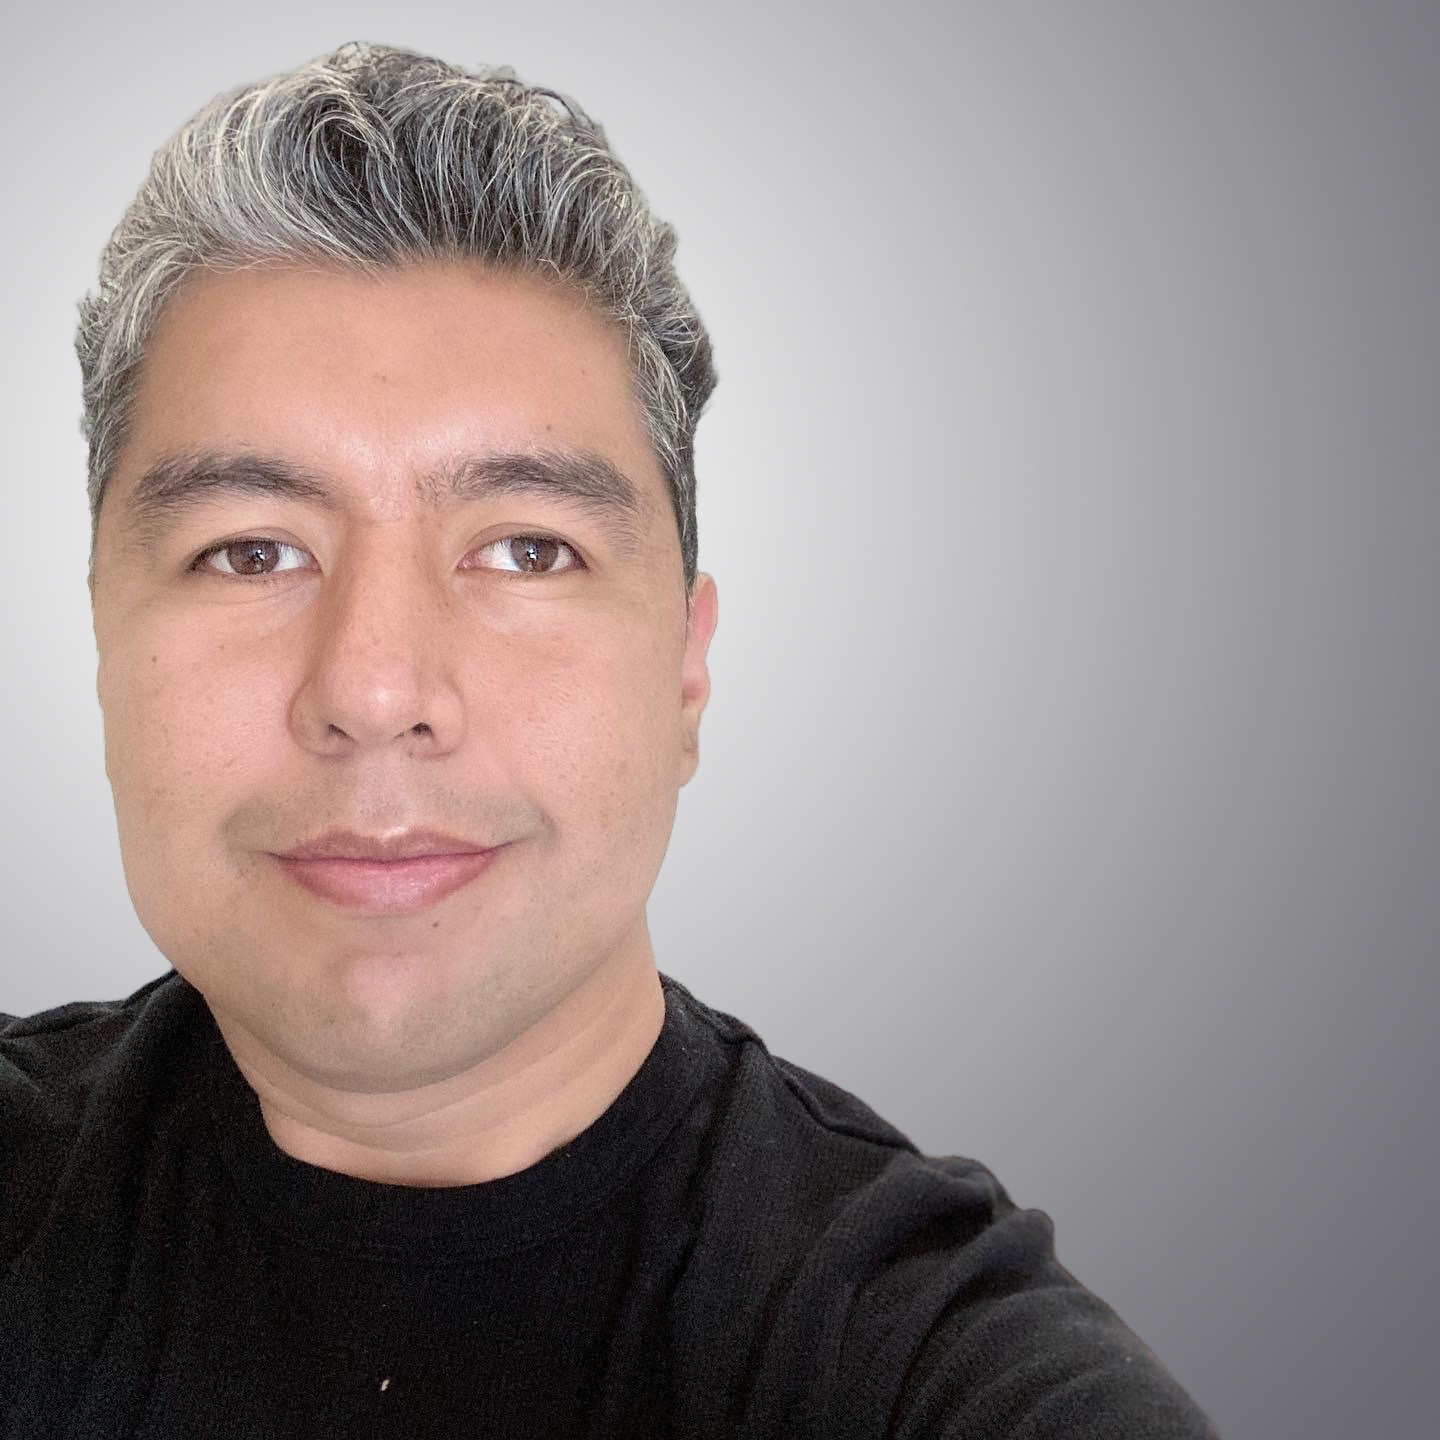
\includegraphics[width=\linewidth]{resources/image.jpg}	%trimming relative to image size

%----------------------------------------------------------------------------------------
%	Habilidades (barra izquierda)
%----------------------------------------------------------------------------------------
\fcolorbox{white}{white}{\begin{minipage}[c][2.4 cm][c]{1\mpwidth}
\LARGE{\textbf{\textcolor{maincol}{Dr. Jes\'us Capistr\'an Mart\'inez}}} \\[2pt]
\end{minipage}} \\
\icontext{CaretRight}{12}{CVU Conahcyt: 377884}{black}\\[6pt]
\icontext{CaretRight}{12}{07 septiembre 1986}{black}\\[6pt]
\icontext{CaretRight}{12}{Mexicano}{black}\\[6pt]
%\icontext{CaretRight}{12}{Soltero}{black}\\[6pt]



\cvsection{Habilidades}


%\cvskill{Recubrimientos \'opticos} {9+ yrs.} {1} \\[-2pt]
 
\cvskill{Desarrollo de celdas solares de pel\'icula delgada} {10+ a\~nos} {1} \\[-2pt]

\cvskill{S\'intesis y caracterizaci\'on de materiales} {8+ a\~nos} {0.9} \\[-2pt]

\cvskill{Divulgaci\'on de la ciencia} {6+ a\~nos} {0.64} \\[-2pt]

\cvskill{Data Science: Python} {5+ yrs.} {0.5} \\[-2pt]

\cvskill{Docencia } {3+ a\~nos} {0.45} \\[-2pt]

\cvskill{Innovaci\'on tecn\'ologica} {2+ a\~nos} {0.3} \\[-2pt]


%----------------------------------------------------------------------------------------
%	Idiomas (barra izquierda)
%----------------------------------------------------------------------------------------

\cvsection{Idiomas}

\cvskill{Espa\~nol} {L1} {1} \\[-2pt]

\cvskill{Ingl\'es} {C1} {0.85} \\[-2pt]


\newpage
%---------------------------------------------------------------------------------------
%	Educaci�n
%---------------------------------------------------------------------------------------
\cvsection{Educaci\'on}

\cvmetaevent
{01/2013 - 08/2017}
{Doctor en Ingenier\'ia: Energ\'ia}
{Universidad Nacional Aut\'onoma de M\'exico (IER-UNAM)}
{\textit{ -- Ciencia de materiales --} \newline Tesis: Celdas solares de pel\'iculas delgadas de Ag-Sb-S.}
\cvmetaevent
{08/2010 - 01/2013}
{Maestro en Ingenier\'ia}
{Universidad Nacional Aut\'onoma de M\'exico (CIE-UNAM)}
{\textit{ -- Ciencia de materiales --} \newline Tesis: Celdas solares con pel\'icula delgada de sulfuro de antimonio.}

\cvmetaevent
{08/2004 - 11/2009}
{Ingeniero Electromec\'anico}
{Instituto Tecnol\'ogico de Zacatepec}
{\textit{ -- Recubrimientos \'opticos --} \newline Memoria de residencia profesional: Desarrollo instrumentaci\'on y evaluaci\'on de un modulo integral de colector solar foto-t\'ermico y controlador de radiaci\'on solar.}

		

\cvsection{Intereses}

\icontext{CaretRight}{12}{Python: Data Analysis}{black}\\[6pt]
\icontext{CaretRight}{12}{LLMs in Education}{black}\\[6pt]
\icontext{CaretRight}{12}{3D-Printing}{black}\\[6pt]





\cvsection{Contacto}

% \icontext{MapMarker}{16}{Ni\~nos H\'eroes No.24\\ Tlaquiltenango Mor. 62980 }{black}\\[6pt]
\iconhref{Home}{16}{www.jesuscapistran.com}{https://jesuscapistran.com}{black}\\[6pt]
\iconemail{Envelope}{16}{capistran@gmail.com}{capistran@gmail.com}{black}\\[6pt]
\icontext{MobilePhone}{16}{ +52 777 188 5442}{black}\\[6pt]
\iconhref{Twitter}{16}{twitter.com/capis}{https://www.twitter.com/capis}{black}\\[6pt]

%\iconhref{Orcid}{16}{orcid.org/0000-0001-8555-5440}{https://www.orcid.org/profile}{black}\\

	
%\cvqrcode{0.3}

\end{leftcolumn}
\begin{rightcolumn}

%---------------------------------------------------------------------------------------
%	TITLE  HEADER
%----------------------------------------------------------------------------------------


%---------------------------------------------------------------------------------------
%	Biografia (resumen)
%---------------------------------------------------------------------------------------

\cvsection{Biograf\'ia}
\vspace{4pt}

%\cvtext{Jes\'us Capistr\'an es especialista en desarrollo de celdas solares de pel\'icula delgada. Cuenta con m\'as de 10 a\~nos de experiencia en laboratorios de s\'intesis y caracterizaci\'on de materiales semiconductores. Su formaci\'on de Ingeniero Electromec\'anico le ha permitido instalar, operar y dar mantenimiento a equipos especializados para el desarrollo de recubrimientos semiconductores. Su especialidad se encuentra en la s\'intesis de pel\'iculas delgadas para su aplicaci\'on en dispositivos fotovoltaicos,  por lo cual es capaz de realizar s\'intesis de materiales semiconductores y \'oxidos met\'alicos  mediante distintas t\'ecnicas de dep\'osito como: dep\'osito qu\'imico,  evaporaci\'on t\'ermica,  sputtering DC/RF y ALD.}
\cvtext{ 
	El Dr. Jesús Capistrán Martínez es un joven investigador que se graduó como ingeniero electromecánico en el Instituto Tecnológico de Zacatepec. Su pasión por la ciencia lo llevó a obtener su doctorado en el Instituto de Energías Renovables de la UNAM, donde se especializó en el desarrollo de celdas solares de película delgada.
	Ha participado en proyectos nacionales como el Centro Mexicano de Innovación en Energía Solar (CEMIE-Sol) y el Laboratorio de Innovación Fotovoltaica y Caracterización de Celdas Solares (LIFYCS), donde ha impulsado el desarrollo de tecnología fotovoltaica 100\% mexicana.
	Actualmente, realiza una estancia postdoctoral en el Instituto de Ciencias de la BUAP, donde desarrolla dipositivos semiconductores para conversión de energia. 

}


%---------------------------------------------------------------------------------------
%	Experiencia laboral 
%---------------------------------------------------------------------------------------

\vspace{10pt}
\cvsection{Experiencia laboral}
\vspace{4pt}


\cvevent
{2021 - actual}
	{Posdoctorado | BUAP}
	{Instituto de Ciencias (Asesor: Dr. Roman Romano) \newline Benem\'erita Universidad Aut\'onoma de Puebla}
	{Proyecto: Desarrollo de celdas solares de heterouni\'on tipo sustrato utilizando calcogenuros de antimonio-plata mediante ba\~no qu\'imico. 
	\begin{itemize}
		\item Prototipo de celda solar flexible sobre sustratos de acero inoxidable.
		\item Puesta en marcha de equipo de laboratorio: Sputtering
	\end{itemize}}
	\vfill\null
	
\cvevent
{2019 - 2020}
	{Posdoctorado | BUAP}
	{Instituto de F\'isica (Asesora: Dra. Mou Pal) \newline Benem\'erita Universidad Aut\'onoma de Puebla}
	{Proyecto: Desarrollo de calcogenuros de metales de pel\'icula delgada y estudio de heterouniones mediante software SCAPS-1D para el dise\~no de dispositivos opto electr\'onicos. 
	\begin{itemize}
		\item Formaci\'on de recurso humano especializado
	\end{itemize}
	}
	\vfill\null

\cvevent
{2017 - 2019}
	{Investigador asociado | CeMIE-Sol P.35}
	{Centro Mexicano de Innovaci\'on en Energ\'ia Solar \newline Universidad Nacional Aut\'onoma de M\'exico (UNAM)}
	{Proyecto: Investigaci\'on y desarrollo de celdas solares con materiales novedosos.
	\begin{itemize}
		\item Prototipo de celda solar con calcogenuro de metales a nivel laboratorio.
		\item Estrateg\'ia de transferencia de tecnolog\'ia. 
	\end{itemize}
	}
	\vfill\null



%---------------------------------------------------------------------------------------
%	Docencia
%---------------------------------------------------------------------------------------

\vspace{5pt}
\cvsection{Docencia}
\vspace{4pt}

\cvevent
{2023}
	{Profesor de asignatura | BUAP}
	{Electricidad y Magnetismo (Maestría)\newline Benem\'erita Universidad Aut\'onoma de Puebla}
	{Actividades: Otoño 2023, curso propedeutico para ingresar a la maestria en Dispositivos Semiconductores de la BUAP. Classroom: \url{https://jesuscapistran.com/courses/2023_electricidad_magnetismo/} }
	\vfill\null

\cvevent
{2023}
	{Profesor de asignatura | BUAP}
	{F\'isica Electr\'onica (Licenciatura)\newline Benem\'erita Universidad Aut\'onoma de Puebla}
	{Actividades: Curso semestral de F\'isica Electr\'onica para alumnos de le Facultad de Ciencias de la Electr\'onica. Classroom: \url{https://jesuscapistran.com/courses/fisica-electronica/} }
	\vfill\null

\cvevent
{2022}
	{Profesor de asignatura | BUAP}
	{Electricidad y Magnetismo (Maestría)\newline Benem\'erita Universidad Aut\'onoma de Puebla}
	{Actividades: Otoño 2022, curso propedeutico para ingreso al programa de maestria del Posgrado en Dispositivos Semiconductores de la BUAP. Classroom: \url{https://jesuscapistran.com/courses/electricidad-y-magnetismo/} }
	\vfill\null

\cvevent
{2021}
	{Profesor de asignatura | BUAP}
	{Mecanica de los Fluidos (Licenciatura)\newline Benem\'erita Universidad Aut\'onoma de Puebla}
	{Actividades: Desarrollo y aplicaci\'on de curso online de Mec\'anica de Fluidos para alumnos de Ingenieria en Energias Renovables. Classroom: \url{https://jesuscapistran.com/courses/mecanica-de-fluidos/} }
	\vfill\null

\cvevent
{2017}
	{Profesor asistente | UNAM}
	{Solar Fotovoltaica (Dr. Karunakaran Nair) \newline Instituto de Energ\'ias Renovables, Temixco, Mor.}
	{Actividades: Asesor\'ia a estudiantes de licenciatura y maestr\'ia para resolver problemas sobre semiconductores y celdas solares.}
	\vfill\null

%
%
%\cvevent
%{2015}
%	{Asistente de laboratorio | UNAM}
%	{Electricidad y Magnetismo (M.I. Jos\'e Ortega) \newline Instituto de Energ\'ias Renovables, Temixco, Mor.}
%	{Actividades: Revisi\'on de practicas de laboratorio y asistencia t\'ecnica a estudiantes de licenciatura en el desarrollo de experimentos.}
%	\vfill\null
%
%
%\cvevent
%{2013}
%	{Profesor asistente | UNAM}
%	{Solar Fotovoltaica (Dr. Antonio J\'imenez) \newline Instituto de Energ\'ias Renovables, Temixco, Mor.}
%	{Actividades: Reuni\'on con estudiantes para resolver problemas relacionados a f\'isica de semiconductores, calificar tareas y ex\'amenes}
%	\vfill\null
%

\vspace{10pt}
\cvsection{Educaci\'on continua}
\vspace{4pt}


\cvevent
{2021 - 2022}
	{Certificaci\'on (330 hrs.) | RENAC (Alemania)}
	{Especialista en Co-beneficios de la Energ\'ia Renovable \newline  Renewables Academy AG, Berlin, Germany}
	{Movilizaci\'on de los Co-beneficios de la Acci\'on Clim\'atica mediante el Desarrollo de Capacidades en las Instituciones de Pol\'iticas Publicas.
	}
	\vfill\null
	
	
	\cvevent
{2022}
	{Curso (20 hrs.) | UNAM }
	{Crash Course de Python y Jupyter Notebook \newline Instituto de Energ\'ias Renovables, Temixco, Mor. }
	{Participaci\'on como asistente en modalidad a distancia del 17 al 21 de enero de 2022, con una duraci\'on de 20 horas.}
	\vfill\null


	\cvevent
{2021}
	{Curso (40 hrs.) | BUAP }
	{M\'etodo Rietveld para Refinamiento Cristalino (XRD)\newline Instituto de F\'isica - Ing. Luis Rivera Terrazas}
	{Participaci\'on como asistente en modalidad a distancia del 17 al 21 de enero de 2022, con una duraci\'on de 20 horas.}
	\vfill\null


%	\cvevent
%{2020}
%	{Curso (2 hrs.) | Equipar, S.A. de C.V. }
%	{ Capacitaci\'on para uso de equipo \newline Instituto de F\'isica - Ing. Luis Rivera Terrazas}
% {Constancia por haber recibido el Curso de Capacitaci\'on para el uso del Equipo: Balanza Anal\'itica Ohaus el dia 17 de febrero de 2020.}
%	\vfill\null
	
	\cvevent
{2019}
	{Taller (20 hrs.) | UNAM }
	{Fabricaci\'on de Celdas Solares de Perovskita Hibrida \newline Instituto de Energ\'ias Renovables, Temixco, Mor. }
	{Diploma por su asistencia al Taller Intensivo de 20 horas: Fabricaci\'on de Celdas Solares de Perovskita H\'ibrida, llevado a cabo del 3 al 7 de junio de 2019.}
	\vfill\null
%	
%
%	\cvevent
%{2018}
%	{Taller (10 hrs.) | UNAM }
%	{Propiedad intelectual: La estrategia de proteger las ideas innovadoras \newline Coordinaci\'on de Innovaci\'on y Desarrollo UNAM }
%	{Constancia por su asistencia al Taller de Propiedad Intelectual, llevado acabo el 23 de agosto de 2018 8:30 a 18:30 hrs. }
%	\vfill\null
%	
%		\cvevent
%{2018}
%	{Curso (24 hrs.) | UNAM }
%	{B\'usqueda en Base de Datos y Redacci\'on de Patentes  \newline Instituto de Energ\'ias Renovables, Temixco, Mor.}
%	{Diploma por su asistencia al curso de 24 hrs. llevado acabo del 29 al 31 de agosto de 2018 }
%	\vfill\null
	
	
%---------------------------------------------------------------------------------------
%	Equipos de laboratorio
%---------------------------------------------------------------------------------------
%---------------------------------------------------------------------------------------
%	Publicaciones
%---------------------------------------------------------------------------------------

\cvsection{Publicaciones}

\begin{itemize}[leftmargin=*]

\item J. Capistr\'an-Mart\'inez, D. Loeza-D\'iaz, D. Mora-Herrera, F. P\'erez-Rodr\'iguez, M. Pal, 2021 Theoretical evaluation of emerging Cd-free $Cu_3BiS_3$ based solar cells using experimental
data of chemically deposited $Cu_3BiS_3$ thin films, \textit{J. Alloys Compd.} 867 (2021) 159156. \url{https://doi.org/10.1016/j.jallcom.2021.159156}

\item J. Capistr\'an-Mart\'inez, M.T.S. Nair, P.K. Nair, Silver Antimony Sulfide Selenide Thin Film Solar Cells via Chemical Deposition, \textit{Phys. Status Solidi.} (2021) pssa.202100058. \url{https://doi.org/10.1002/pssa.202100058}

\item Jesus Capistr\'an-Mart\'inez and P.K. Nair, Photoconductive thin films of $AgSbS_2$ with cubic crystalline structure in solar cells, \textit{Phys. Status Solidi (a)}, 212 (2015) 2869-2876. \url{https://doi.org/10.1002/pssa.201532496}

\item Jes\'us Capistr\'an-Mart\'inez, M.T.S. Nair and P.K. Nair, Silver antimony sulfide-selenide for thin film solar cells, \textit{MRS Proceedings}, 1670, mrss14-1670-e05-11 \url{https://doi.org/10.1557/opl.2014.859}

\item M. Jes\'us Capistr\'an, M.T.S. Nair and P.K. Nair, Antimony sulfide and silver antimony sulfide absorbers for thin film solar cells, \textit{MRS Proceedings}, 1447, \url{https://doi.org/10.1557/opl.2012.1085}

\item P.K. Nair, R. Gonz\'alez Lua, M. Calixto-Rodriguez, J. Capistr\'an-Mart\'inez, O. GomezDaza and M.T.S. Nair, Antimony sulfide absorbers in solar cells, \textit{ECS Transactions}, 41(4), 149-156 (2011), \url{https://doi.org/10.1149/1.3628620}

\item P.K. Nair, Enue Barrios-Salgado, Jes\'us Capistr\'an, Mar\'ia Luisa Ram\'on, M.T.S. Nair and Ralph A. Zingaro, PbS thin films in all-chemically deposited solar cells, \textit{J. Electrochem. Soc.} 157 (2010), D528-D537, \url{https://doi.org/10.1149/1.3467844}
 
\end{itemize}

\vspace{10pt}
\cvsection{Premios}
\vspace{4pt}


\cvevent
{2014}
	{Outstanding contribution}
	{Materials Research Society (MRS)}
	{Award for the outstanding contribution to Symposium E Earth-Abundant Inorganic Solar Energy Conversion, San Francisco, MRS-2014 Spring Meeting.}
	\vfill\null

\cvevent	
{2012}
	{Mejor sesi\'on oral}
	{Centro de investigaci\'on en energ\'ia (CIE-UNAM)}
	{Mejor sesi\'on oral a nivel maestria en el $11^o$ Congreso de estudiantes del Centro de Investigac\'ion en Energ\'ia, Temixco, Mor.}
	\vfill\null

% hofixes to create fake-space to ensure the whole height is used

\mbox{}
\vfill
\mbox{}
\vfill
\mbox{}
\vfill
\mbox{}
\vfill
\mbox{}

 \today     \hspace{1cm}   \hrulefill

\hspace*{30mm}\phantom{Lorem, \today }Jes\'us Capistr\'an Mart\'inez

\end{rightcolumn}
\end{paracol}


\end{document}